\chapter{Network Security and Monitoring}
\section{Security attacks}
\subsection{CDP Reconnaissance Attack}
The Cisco Discovery Protocol (CDP) is a proprietary Layer 2 link discovery protocol. It is enabled on all Cisco devices by default. CDP broadcasts are sent unencrypted and unauthenticated. Therefore, an attacker could interfere with the network infrastructure by sending crafted CDP frames containing bogus device information to directly-connected Cisco devices. \par 
To mitigate the exploitation of CDP, limit the use of CDP on devices or ports. For example, disable CDP on edge ports that connect to untrusted devices. 
\subsection{Telnet Attacks}
There are two types of Telnet attacks:
\begin{itemize}
\item Brute Force Password Attack: The attacker tries to discover the administrative password. 
\item Telnet DoS Attack: The attacker continuously requests Telnet connections in an attempt to render the Telnet service unavailable and preventing an administrator from remotely accessing a switch.
\end{itemize}
\subsection{MAC Address Table Flooding Attack}
MAC address tables are limited in size. MAC flooding attacks exploit this limitation with fake source MAC addresses until the switch MAC address table is full. When the MAC address table becomes full of fake MAC addresses, the switch enters into what is known as fail-open mode. In this mode, the switch broadcasts all frames to all machines on the network. As a result, the attacker can capture all of the frames, even frames that are not addressed to its MAC address table.\par 
Configure \textbf{port security} on the switch to mitigate MAC address table overflow attacks.
\subsection{VLAN Attacks}
The attacker attempts to gain VLAN access by configuring a host to spoof a switch and use the 802.1Q trunking protocol and the Cisco-proprietary Dynamic Trunking Protocol (DTP) feature to trunk with the connecting switch. If successful and the switch establishes a trunk link with the host and the attacker can then access all the VLANS on the switch and hop (i.e., send and receive) traffic on all the VLANs. The best way to prevent basic VLAN attacks:
\begin{itemize}
\item Disable DTP (auto trunking) negotiations on non-trunking ports and non-trunking ports using the \texttt{switchport nonegotiate} interface configuration command. Additionally explicitly force the access ports by using the \texttt{switchport mode access} interface configuration command..
\item Manually enable the trunk link on a trunking port using the switchport mode trunk interface configuration command.
\item Disable DTP (auto trunking) negotiations on trunking   
\item Set the native VLAN to be something other than VLAN 1.
\item Disable unused ports and assign them to an unused VLAN.
\end{itemize}
\subsection{DHCP Attacks}
There are two types of DHCP attacks which can be performed against a switched network: 
\begin{itemize}
\item DHCP spoofing attack: A DHCP spoofing attack occurs when a rogue DHCP server is connected to the network and provides false IP configuration parameters to legitimate clients. Security best practices recommend using DHCP snooping to mitigate DHCP spoofing attacks. 
\item DHCP starvation attack: An attacker floods the DHCP server with bogus DHCP requests and eventually leases all of the available IP addresses in the DHCP server pool. After these IP addresses are issued, the server cannot issue any more addresses, and this situation produces a DoS\footnote{A DoS attack is any attack that is used to overload specific devices and network services with illegitimate traffic, thereby preventing legitimate traffic from reaching those resources.} attack as new clients cannot obtain network access. 
\end{itemize}
	\begin{figure}[hbtp]
	\caption{Trusted and Untrusted ports}\label{DHCPsnooping}
	\centering
	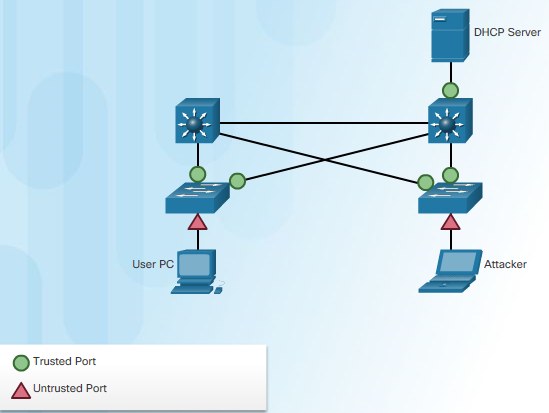
\includegraphics[scale=1]{pictures/DHCPsnooping.PNG}
	\end{figure}
DHCP snooping recognizes two types of ports (see figure \ref{DHCPsnooping}):
\begin{itemize}
\item Trusted DHCP ports: Only ports connecting to upstream DHCP servers should be trusted. These ports should lead to legitimate DHCP servers replying with DHCP Offer and DHCP Ack messages. Trusted ports must be explicitly identified in the configuration.
\item Untrusted ports: These ports connect to hosts that should not be providing DHCP server messages. By default, all switch ports are untrusted.
\end{itemize}
\subsection{Cisco solution}
There are four Cisco switch security solutions to help mitigate Layer 2 attacks:
\begin{itemize}
\item Port security prevents MAC address flooding, DHCP starvation
\item DHCP snooping prevents DHCP spoofing and DHCP starvation
\item DAI (Dynamic ARP inspection) prevents ARP spoofing and ARP poisoning 
\item IPSG (IP Source Guard) prevents MAC and IP address spoofing
\end{itemize}
\subsection{The AAA framework}
The Authentication, Authorization, and Accounting (AAA) framework is used to help secure device access.\par 
An AAA-enabled router uses either the Terminal Access Controller Access Control System (TACACS+) protocol or the Remote Authentication Dial-In User Service (RADIUS) protocol to communicate with the AAA server. While both protocols can be used to communicate between a router and AAA servers, TACACS+ is considered the more secure protocol. This is because all TACACS+ protocol exchanges are encrypted, while RADIUS only encrypts the user’s password. RADIUS does not encrypt user names, accounting information, or any other information carried in the RADIUS message.\par 
Cisco provides two common methods of implementing AAA services:
\begin{itemize}
\item Local AAA Authentication -Local AAA uses a local database for authentication. This method is sometimes known as self-contained authentication. This method stores usernames and passwords locally in the Cisco router, and users authenticate against the local database. Local AAA is ideal for small networks.
\item Server-Based AAA Authentication - Server-based AAA authentication is a much more scalable solution. With server-based method, the router accesses a central AAA server. The AAA server contains the usernames and password for all users and serves as a central authentication system for all infrastructure devices.
\end{itemize}
\subsection{802.1X}
The IEEE 802.1X standard defines a port-based access control and authentication protocol. IEEE 802.1X restricts unauthorized workstations from connecting to a LAN through publicly accessible switch ports. 
	\begin{figure}[hbtp]
	\caption{802.1X roles}\label{8021X}
	\centering
	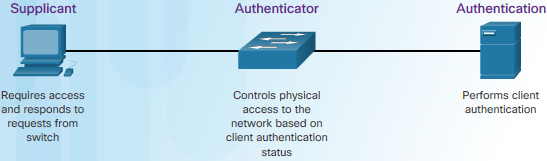
\includegraphics[ width=0.8\textwidth ]{pictures/8021X.PNG}
	\end{figure}
With 802.1X port-based authentication, the devices in the network have specific roles, as shown in the figure \ref{8021X}:
\begin{itemize}
\item Client (Supplicant): The device is a PC running 802.1X-compliant client software.
\item Switch (Authenticator): This controls physical access to the network based on the authentication status of the client. The switch requests identifying information from the client, verifies that information with the authentication server, and relays a response to the client.
\item Authentication server: validates the identity of the client and notifies the switch or other authenticator such as a wireless access point whether the client is authorized to access the LAN and switch services.
\end{itemize}
\section{SNMP}
\subsection{Introduction to SNMP}
Simple Network Management Protocol (SNMP) was developed to allow administrators to manage nodes such as servers, workstations, routers, switches, and security appliances, on an IP network.
The SNMP system consists of three elements:
\begin{itemize}
\item \textbf{SNMP manager}: is part of a network management system (NMS), run SNMP management software. 
\item \textbf{SNMP agents} (managed node):  responsible for providing access to the local MIB. The SNMP agent and MIB reside on SNMP client devices.
\item \textbf{MIB} (Management Information Base): store data about the device and operational statistics 
\end{itemize}
\subsection{SNMP operation}
\subsubsection{SNMP requests}
The SNMP manager uses the get and set actions to perform the operations described in the table in Figure \ref{SNMPoperation}.
	\begin{figure}[hbtp]
	\caption{SNMP operations}\label{SNMPoperation}
	\centering
	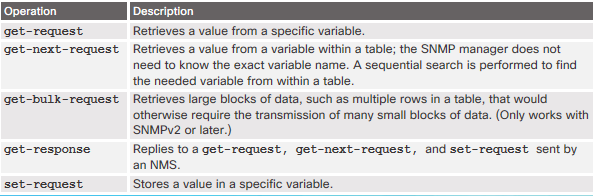
\includegraphics[scale=1]{pictures/SNMPoperation.PNG}
	\end{figure}
\subsubsection{SNMP Agent Traps}
An NMS periodically polls the SNMP agents residing on managed devices, by querying the device for data using the get request. Using this process, a network management application can collect information to monitor traffic loads and to verify device configurations of managed devices.\par 
Periodic SNMP polling does have disadvantages. First, there is a delay between the time that an event occurs and the time that it is noticed (via polling) by the NMS. Second, there is a trade-off between polling frequency and bandwidth usage.\par 
To mitigate these disadvantages, it is possible for SNMP agents to generate and send traps to inform the NMS immediately of certain events. Traps are unsolicited messages alerting the SNMP manager to a condition or event on the network. 
\subsubsection{Community string}
SNMPv1 and SNMPv2c use community strings that control access to the MIB. Community strings are plaintext passwords. There are two types of community strings: Read-only (\textbf{ro}) and Read-write (\textbf{rw}).
\subsubsection{object ID}
MIB saves data in variables and organizes them hierarchically. Formally, the MIB defines each variable as an object ID (OID). OIDs uniquely identify managed objects in the MIB hierarchy (figure \ref{OID-tree}).
	\begin{figure}[hbtp]
	\caption{OID tree}\label{OID-tree}
	\centering
	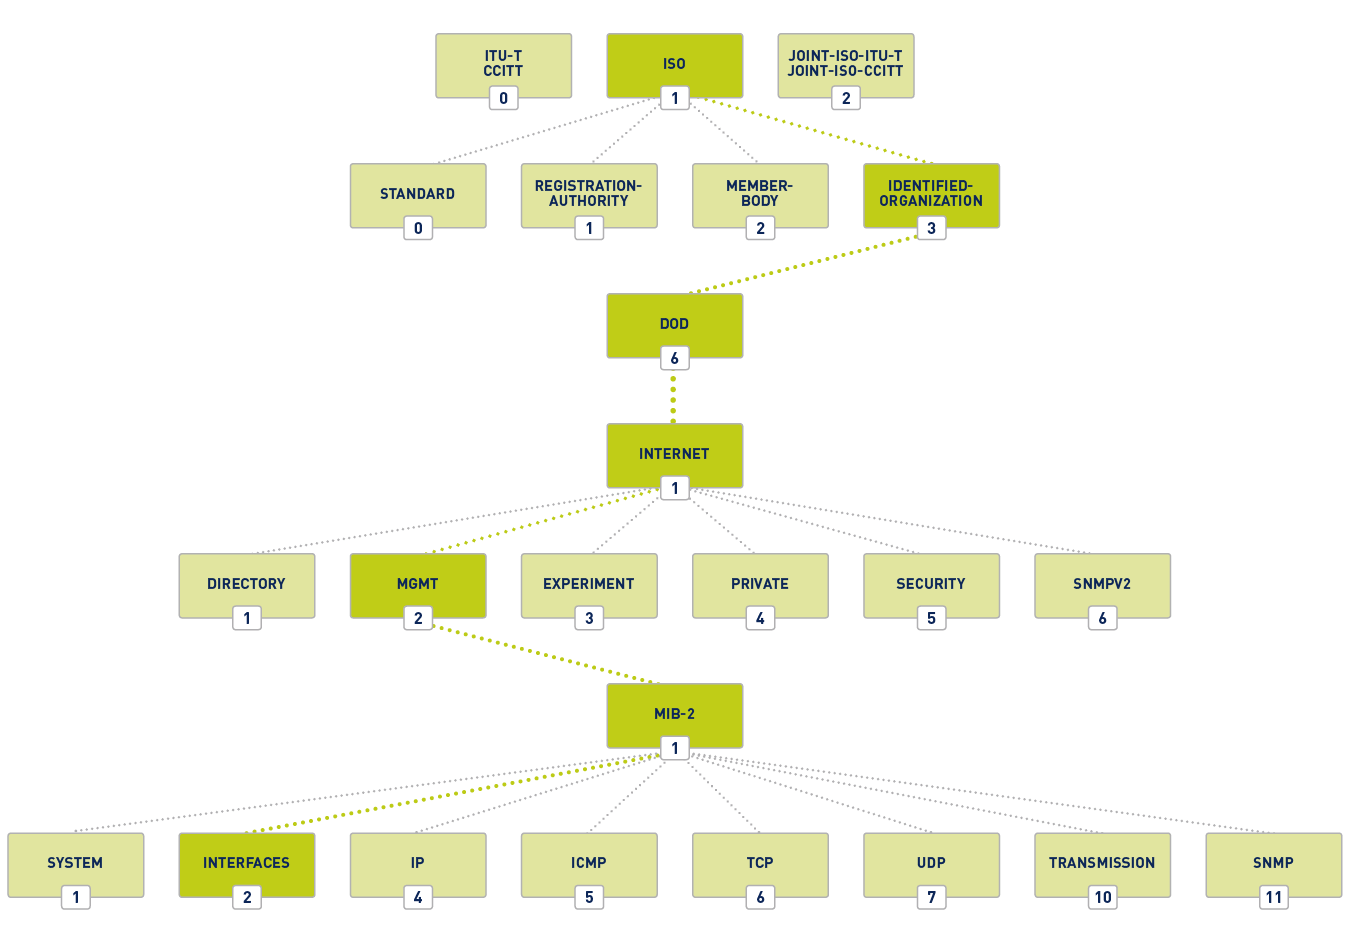
\includegraphics[scale=1]{pictures/OID-tree.png}
	\end{figure}
For example, OIDs belonging to Cisco, are numbered as follows: .iso (1).org (3).dod (6).internet (1).private (4).enterprises (1).cisco (9). Therefore the OID is 1.3.6.1.4.1.9.
The data is retrieved via the snmpget utility, issued on the NMS. Using the snmpget utility, one can manually retrieve real-time data or have the NMS run a report which would give you a period of time that you could use the data to get the average. 
\section{SNMP configuration}
\subsection{SNMPv2}
\begin{listing}
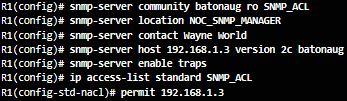
\includegraphics[scale=1]{pictures/SNMPv2.PNG} 
\end{listing}
\begin{enumerate}
\item (Required) Configure the community string and access level (read-only or read-write) with the snmp-server community string ro | rw command.

\item (Optional) Document the location of the device using the snmp-server location text command.

\item (Optional) Document the system contact using the snmp-server contact text command.

\item (Optional) Restrict SNMP access to NMS hosts (SNMP managers) that are permitted by an ACL: define the ACL and then reference the ACL with the snmp-server community string access-list-number-or-name command. This command can be used both to specify a community string and to restrict SNMP access via ACLs. Step 1 and Step 4 can be combined into one step, if desired; the Cisco networking device combines the two commands into one if they are entered separately.

\item (Optional) Specify the recipient of the SNMP trap operations with the snmp-server hosthost-id [version {1| 2c | 3 [auth | noauth | priv]}] community-string command. By default, no trap manager is defined.

\item (Optional) Enable traps on an SNMP agent with the snmp-server enable traps notification-types command. If no trap notification types are specified in this command, then all trap types are sent. Repeated use of this command is required if a particular subset of trap types is desired.
\end{enumerate}
\note To verify SNMP configuration, use any of the variations of the \texttt{show snmp} command.\\ \note Only the first step is required, the rest are optional.\\
\note By default, SNMP does not have any traps set. Without this command, SNMP managers must poll for all relevant information. 
\subsection{SNMPv3}
SNMPv3 provides three security features: Message integrity and authentication, Encryption, Access control. SNMPv3 can be secured with the four steps.\\
\begin{listing}
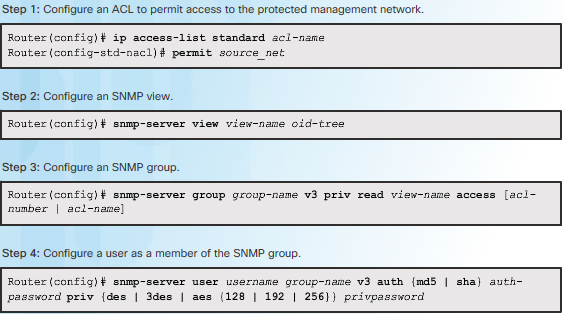
\includegraphics[scale=1]{pictures/SNMPv3steps.PNG} 
\end{listing}

\begin{verbatim}
1	R1(config)# ip access-list standard PERMIT-ADMIN
2	R1(config-std-nacl)# permit 192.168.1.0 0.0.0.255
3	R1(config-std-nacl)# exit
4	R1(config)# snmp-server view SNMP-RO iso included
5	R1(config)# snmp-server group ADMIN v3 priv read SNMP-RO access PERMIT-ADMIN
6	R1(config)# snmp-server user BOB ADMIN v3 auth sha cisco12345 priv aes 128 cisco54321
7	R1(config)# end
\end{verbatim}
\begin{description}
\item[line 1,2] The above example configures a standard ACL named PERMIT-ADMIN. 
\item[line 4] An SNMP view is named SNMP-RO and is configured to include the entire ISO tree from the MIB. 
\item[line 5] An SNMP group is configured with the name ADMIN. SNMP is set to version 3 with authentication and encryption required. The group is allowed read-only access to the view SNMP-RO. Access for the group is limited by the PERMIT-ADMIN ACL. 
\item[line 6] An SNMP user, BOB, is configured as a member of the group ADMIN. Authentication is set to use SHA, and an authentication password is configured. Although R1 supports up to AES 256 encryption, the SNMP management software only supports AES 128. Therefore, the encryption is set to AES 128 and an encryption password is configured.
\end{description}

\section{SPAN}
\subsection{Introduction}
A packet analyzer is typically software that captures packets entering and exiting a network interface card (NIC). However, the basic operation of a modern switched network disables the packet analyzer ability to capture traffic from other sources. For instance, a user running Wireshark can only capture traffic going to their NIC.\par 
The solution to this dilemma is to enable port mirroring. The port mirroring feature allows a switch to copy and send Ethernet frames from specific ports to the destination port connected to a packet analyzer. The Switched Port Analyzer (SPAN) feature on Cisco switches is a type of port mirroring that sends copies of the frame entering a port, out another port on the same switch.\par 
SPAN is commonly implemented to deliver traffic to specialized devices including: Packet analyzers (such as Wireshark) and IPSs (Intrusion Prevention Systems)
\subsection{Local SPAN}
Local SPAN is when traffic on a switch is mirrored to another port on that switch. A SPAN session is the association between source ports (or VLANs) and a destination port. Traffic entering or leaving the source port (or VLAN) is replicated by the switch on the destination port. There are three important things to consider when configuring SPAN:
\begin{itemize}
\item The destination port cannot be a source port, and the source port cannot be a destination port.
\item The number of destination ports is platform-dependent. Some platforms allow for more than one destination port.
\item The destination port is no longer a normal switch port. Only monitored traffic passes through that port.
\end{itemize}
\begin{verbatim}
S1(config)# monitor session 1 source interface f0/1
S1(config)# monitor session 1 destination interface f0/2
S1(config)# end
S1# show monitor
\end{verbatim}
The above command is used to associate a source port and a destination port with a SPAN session. A separate monitor session command is used for each session. A VLAN can be specified instead of a physical port. Use \texttt{show monitor} to verify SPAN configuration.\par
	\begin{figure}[hbtp]
	\caption{Verifying SPAN}\label{SPAN}
	\centering
	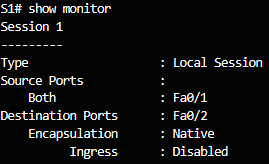
\includegraphics[scale=0.8]{pictures/SPAN.PNG}
	\end{figure}
In the output of show command shown in Figure \ref{SPAN}, the session number is 1, the source port for both traffic directions (receive and transmit) is F0/1, and the destination port is F0/2. The ingress SPAN is disabled on the destination port, so only traffic that leaves the destination port is copied to that port.
\subsection{RSPAN}
Remote SPAN (RSPAN) allows source and destination ports to be in different switches. RSPAN uses two sessions. One session is used as the source and one session is used to copy or receive the traffic from a VLAN. The traffic for each RSPAN session is carried over trunk links in a user-specified RSPAN VLAN that is dedicated (for that RSPAN session) in all participating switches. 